\section{Durchführung}
\label{sec:Durchführung}

Ein Schema des Aufbaus ist in Abbildung \ref{fig:Schema} zu sehen.
Zunächst werden Laser, Spalt und Photoelement ausgerichtet.
Dabei wird der Abstand $L$ zwischen Spalt und Photoelement ausgemessen.
Vor der eigentlichen Messung wird der Dunkelstorm gemessen, der durch die Umgebungsbeleuchtung entsteht
und um den die späteren Messwerte korrigiert werden müssen.
Zur Vermessung des Beugungsbildes wird der Verschiebereiter im Millimeter-Bereich verschoben und
der Strom als Maß der Intensität mit der entsprechenden Position notiert.
Die Messung wird für einen Einzelspalt und zwei verschiedene Doppelspalte durchgeführt.
\begin{figure}
  \centering
  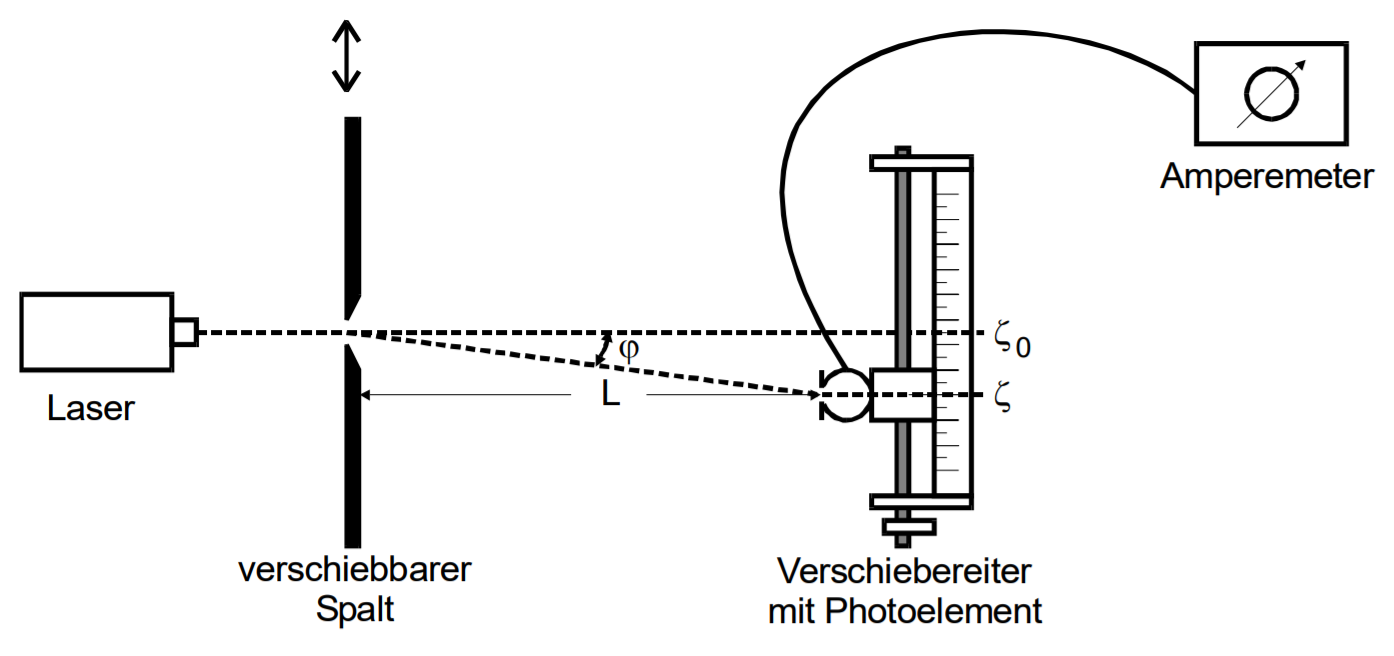
\includegraphics[height=6cm]{data/Schema.png}
  \caption{Versuchsanordnung zur Messung des Beugungsbildes. \cite{sample}}
  \label{fig:Schema}
\end{figure}
